	\subsection{Taxonomy of mobile virtualization techniques by \textit{Shuja}}
	
	\begin{figure}[H]
		\centering
		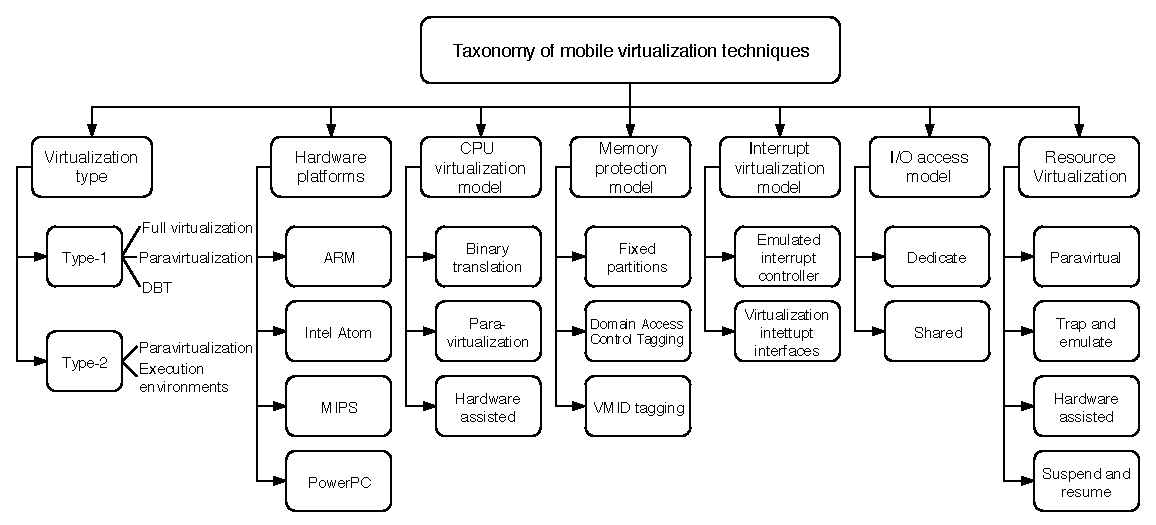
\includegraphics[width=8.5cm]{images/Shuja2016.pdf}
		\vspace{-0.2cm}
		\caption{Taxonomy of mobile virtualization techniques by \textit{Junaid Shuja, Kashif Bilal, Abdullah Gani and Samee Ullah Khan} in 2016 \cite{Shuja2016}.}
		\label{fig:TaxonomyByShuja}
	\end{figure}

	The study by Shuja et al \cite{Shuja2016} focuses on a taxonomy of mobile virtualization techniques with seven main categories: \textit{Virtualization type}, \textit{Hardware platforms}, \textit{CPU virtualization model}, \textit{Memory protection model}, \textit{Interrupt virtualization model}, \textit{I/O access model} and finally \textit{Network virtualization model}.
	
	
	
	
	
	